\documentclass[11pt,twoside,a4paper]{article}
\usepackage{german,a4wide,amsmath,amssymb}

% Mann will direkt Umlaute eingeben k�nnen statt \"a, \"o, \"u usw.
% Entweder:
%\usepackage[latin1]{inputenc}
% oder:
%\usepackage{umlaut}


% Trennvorschl"age (in {} einfuegen, wenn nicht automatisch getrennt wird:
% z.B. Authen-ti-ka-tions-sys-tem)
\hyphenation{}

\hyphenation{min-des-tens}
\hyphenation{Per-for-mance}
\hyphenation{Com-pu-ting}



%-------------------------- Formatsachen --------------------------%

% Bild-, Tabellenunterschriften veraendern:
% Nummer fett, kleinerer Text fuer Bildunterschrift
\usepackage[bf,small]{caption}

\usepackage{mathpazo}  % -- Palatino als Zeichensatz -- einfach diese
					   % Zeile auskommentieren, falls nicht installiert
%\usepackage{mathptmx}  % -- Times als Zeichensatz

% Zum Unterscheiden von Entwurfs- und endgueltiger Fassung
%\usepackage{draftcopy}
%\draftcopySetGrey{0.90}   %   90% = sehr helles Grau
%\draftcopyName{ENTWURF}{155}   % statt ``DRAFT''
%\draftcopySetScale{1}

%--------------- Zeilen- und Absatzabstaende ----------------------%
\setlength{\parindent}{0em}
\setlength{\parskip}{\medskipamount}    % Abstand zwischen Abs"atzen

% ---------- Umgebungen f"ur Satz/ Lemma, etc. --------------------%
\newtheorem{satz}{Satz}
\newtheorem{nota}{Notation}
\newtheorem{defi}{Definition}
\newtheorem{kons}{Konstruktion}

\newenvironment{notation}{\noindent \textbf{Notation: }}{}
\newenvironment{beweis}{\noindent \textbf{Beweis: }}{}
\newenvironment{anmerkung}{\noindent \textbf{Anmerkung: }}{}
\newenvironment{anmerkungen}{\noindent \textbf{Anmerkungen: }}{}
\newenvironment{beispiel}{\noindent \textbf{Beispiel: }}{}
\newenvironment{beispiele}{\noindent \textbf{Beispiele: }}{}

% URLs und Mailadressen etc. richtig trennen:
\usepackage{url}
% Auch praktisch fuer Mailadressen: \url{blabla@laberlaber.de}

% --------------------- Eigene Befehle fuer math. Mengen ---------%
\newcommand{\N}{{\rm I\!N}}             % die natuerlichen Zahlen
\newcommand{\Z}{\mathbb{Z}}             % fuer ganze Zahlen
\newcommand{\R}{\mathbb{R}}             % die reellen Zahlen
\newcommand{\Prim}{{\rm I\!P}}          % die Primzahlen


% -- Sinnvolle Befehle, um sich selbst Notizen im Text zu machen --%

% "Ungeordnete Gedanken, die noch irgendwo reinsollen":
\newcommand{\kramsubsection}[1][Unsortierte Textfragmente]{%
\subsection*{#1}%
\addcontentsline{toc}{subsection}{#1}%
}

% Randbemerkung:
\newcommand{\bemerkung}[1]{\marginpar{\small\textsl{\textsf{#1}}}}

% "Hier muss noch [weiter-]geschrieben werden" (Baustellensymbol am Rand)
%
% [Damit dieser Befehl funktioniert, muss man natuerlich erstmal
%  das Icon "Baustelle.eps" besorgen!!  Also entweder selbermachen
%  oder downloaden:
%  http://www.net.in.tum.de/teaching/WS04/routing/Baustelle.eps.gz  ]
\newcommand{\baustelle}[1][]{
 \marginpar{%
   \centerline{\includegraphics[scale=0.3]{Baustelle.eps}}
   {\small\textsl{\textsf{\raggedright #1}}}
}}

\usepackage{graphicx}
\usepackage{subcaption}
\usepackage{wrapfig}


\begin{document}

\title{Seminararbeit \\
\small GPUDirect MPI Communications and Optimizations to Accelerate FFTs on Exascale Systems}
\author{Robert Graf, Tobias Seitz\\
%  (\texttt{fridolw@in.tum.de})\\[5mm]
%  Seminar "`Internetrouting"' , \\
  Ostbayerische Technische Hochschule Regensburg
}
  
\date{WS\, 2019/2020 (Version vom \today)}

\maketitle


\abstract{Dieses Papier behandelt die Umsetzung der 3-dimensionalen Fast-Fourier-Transformation in Multi-Grafikprozessorsystemen in einem High-Performance-Computing Kontext. Dabei werden die algorithmischen Methoden selbst, die Beschleunigung durch verwendete Hardware und die Behandlung von Problemen bei der Umsetzung auf einer Multi-Prozessor-Systemarchitektur behandelt.}


\section{Einleitung}

Die Schnelle Fourier-Transformation (eng. \textit{fast fourier-transform (FFT)})ist eine der wichtigsten Operationen in der Signalverarbeitung. Mit ihr kann ein durch Amplitude angegebenes Signal in den Frequenzbereich transformiert werden. Dabei werden die enthaltenen Frequenzen im Ursprungssignal erkennbar.\\
Sie findet daher Anwendung in Wissenschaft und Industrie in Bereichen wie Natursimulation, Maschinellem Lernen, Fabrikation, Ingenieurswesen oder Signalmodulation.\\
Die Umsetzung im speziellen der 3D-FFT auf hochparallelen Grafikprozessoren kann enorme Beschleunigungen in der Berechnungszeit erbringen.
Durch die effiziente Umsetzung im Speziellen in einer Multi-Prozessor-Umgebung sollen größere Inputdimensionen performant erschlossen werden. Durch die GPU-Beschleunigung und den verwendeten Systemen treten jedoch inhärente Problemstellungen auf, zu denen Lösungsansätze vorgestellt werden sollen.\\









\section{FFT}

Die schnelle Fourier-Transformation (FFT) ist ein Algorithmus von  James Cooley und John W. Tukey zur schnellen Berechnung der diskreten Fourier-Transformation. Mit dieser Transformation kann ein zeitdiskretes Signal $f(t)$ in ihre Frequenzanteile bzw. Frequenzspektrum zerlegt werden \cite[S.14]{hejobu 84}. Ein Frequenzspektrum beschreibt die Stärke der jeweiligen Frequenz im zu Grunde liegenden Signal. Um den FFT-Algorithmus zu verstehen, müssen kurz ein paar Grundlagen erklärt werden.


\subsection{Fourierreihe}

Die Fourierreihe ist eine Reihenentwicklung ähnlich der Taylor-Serie, die periodische Funktionen als eine unendlich Reihe von Sinus- und Cosinus-Funktionen beliebig genau approximiert kann \cite[K. 11.4]{krenor 11}. Eine periodische Funktion muss sich in Periode T wiederholen. Dem entsprechend muss gelten:
\begin{equation}
f(t) = f(t + T)
\end{equation}

Die Fourierserie besitzt folgende Form:
\begin{equation}
f(t) = \frac{a_0}{2} + \sum_{n=1}^{\infty} a_n cos \left( \frac{n2 \pi t}{T} \right) + b_n sin \left( \frac{n2 \pi t}{T} \right)
\label{eq:fourierreihe}
\end{equation}
Für die Approximation müssen die Koeffizienten $a_n$ und $b_n$ berechnet werden (für die Berechnung siehe \cite[K. 11.2]{krenor 11}). Die Koeffizienten $a_n$ und $b_n$ stehen dabei im Zusammenhang mit der Amplitude der verschiedenen Frequenzen in der Reihe \cite[K. 2.5]{scho 05}. Somit lässt sich eine periodische Funktion $f(t)$ mit der Fourierreihe in ihre Teilfrequenzen zerlegen und mit Hilfe der Koeffizienten das Frequenzspektrum anzeigen lassen (siehe Abbildung \ref{fig:fourierreihe}).
\newline
Die Entwicklung einer Funktion $f(t)$ kann auch als Zerlegung der Funktion in die durch trigonometrischen Basisfunktionen dargestellten Schwingungen verstanden werden und heißt Fourieranalyse.
\begin{figure}
\centering
 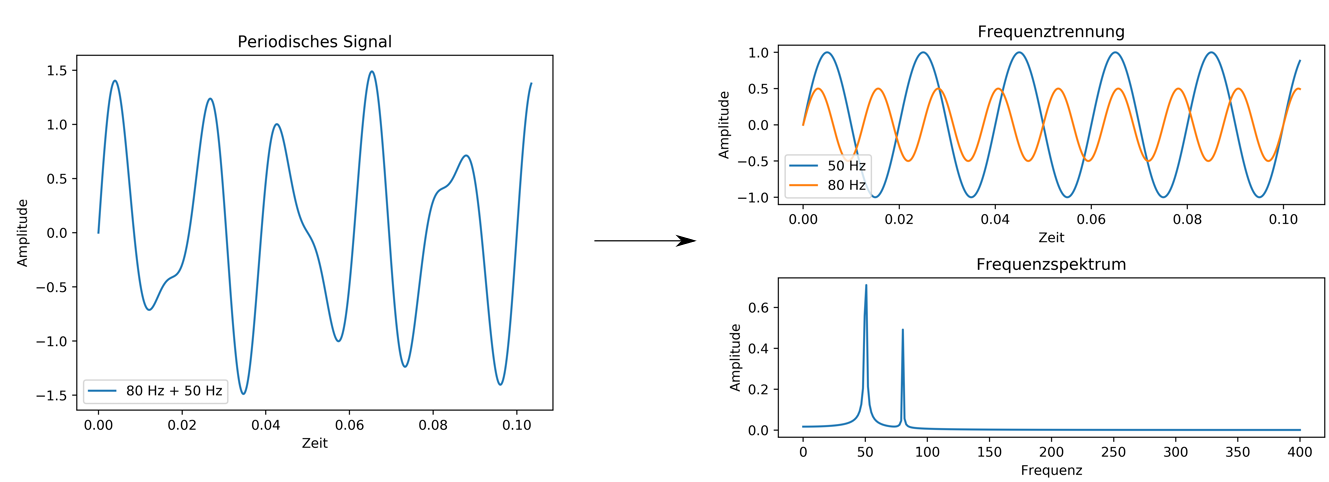
\includegraphics[width=0.8\textwidth]{Pictures/Fourierreihe.png}
\caption{Anwendung Fourierreihe}
\label{fig:fourierreihe}
\end{figure} 
\newline
Für die Fourierreihe gibt es auch eine komplexe Darstellung. Für diese muss zuerst die eulersche Formel $e^{ix} = cos(x) + i sin(x)$ umgestellt werden:
\begin{equation}
cos(x) = \frac{e^{ix} + e^{-ix}}{2}
\label{eq:euler1}
\end{equation}
\begin{equation}
sin(x) = \frac{e^{ix} - e^{-ix}}{2i}
\label{eq:euler2}
\end{equation}
Nun müssen die trigonometrischen Funktion in Formel \ref{eq:fourierreihe} mit Formel \ref{eq:euler1} und \ref{eq:euler2} ersetzt werden.
Dabei entsteht folgende Gleichung:
\begin{equation}
f(x) = \sum_{n=-\infty}^{\infty} c_{n} e^{in2\pi x / T}
\label{FS}
\end{equation}
Hierbei ist $c_n$ eine Konstante, die für die Approximation der Fourier berechnet werden muss.


\subsection{Diskrete Fouriertransformation}
Die diskrete Fouriertransformation DFT verwandelt wie die Fourierserie ein periodische Signal in ihr Frequenzspektrum um. Im Gegensatz zur Fourierreihe wird aber ein endliches zeitdiskretes Signal und kein kontinuierliches Signal verwandelt.
Deswegen ist die DFT auch besser für Algorithmen in der Informatik geeignet, da Rechner mit diskreten Werten arbeiten. Folgende Formel zeigt wie ein zeitdiskretes Signal $x_{n} = x_{1}, x_{2},...$ in ein diskretes, periodisches Frequenzspektrum $X_{k} = X_{1}, X_{2},...$ transformiert wird \cite[S.17]{and 12}:
\begin{equation}
X_{k}= \sum_{n=0}^{N-1} x_{n} e^{-i2 \pi kn /N} \text{  für } k=0,...,N-1
\label{eq:DFT}
\end{equation}

Die inverse DFT (iDFT) lautet \cite[S.20]{and 12}:
\begin{equation}
x_{k}= \frac{1}{N}\sum_{k=0}^{N-1} X_{k} e^{i2 \pi kn /N} \text{  für }  n=0,...,N-1
\label{idft}
\end{equation}
Beide Formeln lassen sich aus der komplexen Formel \ref{FS} der Fourierreihe herleiten \cite[S. 77-79]{ser 17}. Die DFT lässt sich mit Hilfe der Einheitswurzel $w_{N} = e^{-2 \pi ik /N}$ in folgende Formel vereinfachen:
\begin{equation}
X_{k}= \sum_{n=0}^{N-1} x_{n} w_{N}^{kn}
\end{equation}
Mit Hilfe der Fouriermatrix $F_{N} = (w^{kn})_{k,n=0}^{N-1}$ und der Matrixschreibweise erhalten wir folgende Formel:
\begin{equation}
X_{k} = x_{n}F_{N}
\label{eq:dft fouriermatrix}
\end{equation}
Somit ist die DFT eine Matrix-Vektor-Multiplikation zwischen einem Vektor $x_n$ und der $n*n$ Fouriermatrix.
Somit benötigt die DFT für n Elemente jeweils n Multiplikationen und für jede Multiplikation n - 1 Additionen. Es ergibt sich folgende Laufzeit: 
\begin{equation}
DFT \in \mathcal O(n^2)
\end{equation}

\subsection{Implementierung FFT}
Die schnelle Fouriertransformation FFT ist ein Algorithmus für die DFT, der durch Ausnutzen der Symmetrie der Einheitswurzel die Laufzeit des Algorithmus auf $FFT \in \mathcal O(n \log n)$ verringert.
\newline
Nach Formel \ref{eq:dft fouriermatrix} ist die DFT eine Matrix-Vektor-Multiplikation aus $x_{n}$ und der Fouriermatrix $F_{N}$:
\begin{equation}
\left( \begin{array}{cccc}
w^0 & w^0 & \cdots & w^0\\
w^0 & w^1 & \cdots & w^{N-1}\\
\vdots & \vdots & \ddots & \vdots\\
w^0 & w^{N-1} & \cdots & w^{(N-1)(N-1)}\\
\end{array}\right)
\left( \begin{array}{c}
x_0\\
x_1\\
\vdots\\
x_{N-1}
\end{array}\right)
\end{equation}
Die Idee des Verfahrens ist es die Matrix-Vektor-Multiplikation mit $N$ Elemente auf zwei Matrix-Vektor-Multiplikation mit $\frac{N}{2}$ aufzuteilen. Durch diese Aufteilung werden Rechenoperationen eingespart. Dieser Vorgang wird solange wiederholt bis nur noch ein Element in der Matrix ist. Deswegen muss $N$ eine Zweierpotenz sein. Der Algorithmus ist somit ein Teile-Herrsche-Verfahren.
Für das Aufteilen muss die Struktur der Fouriermatrix vereinfacht werden. Dies ist durch folgende Eigenschaften der $N$-ten Einheitswurzel möglich:
\begin{itemize}
\item $w^{N/2} = -1$ \text{ für $N$ gerade}
\item $w^{kN} = 1$
\end{itemize}
Zur Veranschaulichung wird der erste Schritt im Verfahren an einer $8*8$ Fouriermatrix durchgeführt:
\begin{equation*}
\left( \begin{array}{cccccccc}
w^{0} & w^{0} & w^{0} & w^{0} & w^{0} & w^{0} & w^{0} & w^{0}\\
w^{0} & w^{1} & w^{2} & w^{3} & w^{4} & w^{5} & w^{6} & w^{7}\\
w^{0} & w^{2} & w^{4} & w^{6} & w^{8} & w^{10} & w^{12} & w^{14}\\
w^{0} & w^{3} & w^{6} & w^{9} & w^{12} & w^{15} & w^{18} & w^{21}\\
w^{0} & w^{4} & w^{8} & w^{12} & w^{16} & w^{20} & w^{24} & w^{28}\\
w^{0} & w^{5} & w^{10} & w^{15} & w^{20} & w^{25} & w^{30} & w^{35}\\
w^{0} & w^{6} & w^{12} & w^{18} & w^{24} & w^{30} & w^{36} & w^{42}\\
w^{0} & w^{7} & w^{14} & w^{21} & w^{28} & w^{35} & w^{42} & w^{49}\\
\end{array} \right)
\end{equation*}
In Zeile 3, 5 und 7 kann in der rechten Hälfte die Eigenschaft $w^{kN} = 1$ ausgenutzt werden:
\begin{equation}
\left( \begin{array}{cccccccc}
w^{0} & w^{0} & w^{0} & w^{0} & w^{0} & w^{0} & w^{0} & w^{0}\\
w^{0} & w^{1} & w^{2} & w^{3} & w^{4} & w^{5} & w^{6} & w^{7}\\
w^{0} & w^{2} & w^{4} & w^{6} & w^{0} & w^{2} & w^{4} & w^{6}\\
w^{0} & w^{3} & w^{6} & w^{9} & w^{12} & w^{15} & w^{18} & w^{21}\\
w^{0} & w^{4} & w^{8} & w^{12} & w^{0} & w^{4} & w^{8} & w^{12}\\
w^{0} & w^{5} & w^{10} & w^{15} & w^{20} & w^{25} & w^{30} & w^{35}\\
w^{0} & w^{6} & w^{12} & w^{18} & w^{0} & w^{6} & w^{12} & w^{18}\\
w^{0} & w^{7} & w^{14} & w^{21} & w^{28} & w^{35} & w^{42} & w^{49}\\
\end{array} \right)
\end{equation}
In Zeile 1, 3, 5 und 7 ist die linke Hälfte gleich der rechten Hälfte.
Im nächsten Schritt wird die rechte Hälfte der Zeilen 2, 4, 6 und 8 mit der Eigenschaft $w^{kN} = 1$ vereinfacht:
\begin{equation*}
\left( \begin{array}{cccccccc}
w^{0} & w^{0} & w^{0} & w^{0} & w^{0} & w^{0} & w^{0} & w^{0}\\
w^{0} & w^{1} & w^{2} & w^{3} & w^{4} & w^{5} & w^{6} & w^{7}\\
w^{0} & w^{2} & w^{4} & w^{6} & w^{0} & w^{2} & w^{4} & w^{6}\\
w^{0} & w^{3} & w^{6} & w^{9} & w^{4} & w^{7} & w^{10} & w^{13}\\
w^{0} & w^{4} & w^{8} & w^{12} & w^{0} & w^{4} & w^{8} & w^{12}\\
w^{0} & w^{5} & w^{10} & w^{15} & w^{4} & w^{9} & w^{14} & w^{19}\\
w^{0} & w^{6} & w^{12} & w^{18} & w^{0} & w^{6} & w^{12} & w^{18}\\
w^{0} & w^{7} & w^{14} & w^{21} & w^{4} & w^{11} & w^{18} & w^{25}\\
\end{array} \right)
\end{equation*}
Im letzten Schritt wird in den Zeile 2, 4, 6 und 8 die Eigenschaft $w^{N/2} = -1$ benutzt und die Potenzen geschickt aufgeteilt:
\begin{equation*}
\left( \begin{array}{cccccccc}
w^{0} & w^{0} & w^{0} & w^{0} & w^{0} & w^{0} & w^{0} & w^{0}\\
w^{0}w^{0} & w^{1}w^{0} & w^{2}w^{0} & w^{3}w^{0} & -w^{0}w^{0} & -w^{1}w^{0} & -w^{2}w^{0} & -w^{3}w^{0}\\
w^{0} & w^{2} & w^{4} & w^{6} & w^{0} & w^{2} & w^{4} & w^{6}\\
w^{0}w^{0} & w^{1}w^{2} & w^{2}w^{4} & w^{3}w^{6} & -w^{0}w^{0} & -w^{1}w^{2} & -w^{2}w^{4} & -w^{3}w^{6}\\
w^{0} & w^{4} & w^{8} & w^{12} & w^{0} & w^{4} & w^{8} & w^{12}\\
w^{0}w^{0} & w^{1}w^{4} & w^{2}w^{8} & w^{3}w^{12} & -w^{0}w^{0} & -w^{1}w^{4} & -w^{2}w^{8} & -w^{3}w^{12}\\
w^{0} & w^{6} & w^{12} & w^{18} & w^{0} & w^{6} & w^{12} & w^{18}\\
w^{0}w^{0} & w^{1}w^{6} & w^{2}w^{12} & w^{3}w^{18} & -w^{0}w^{0} & -w^{1}w^{6} & -w^{2}w^{12} & -w^{3}w^{18}\\
\end{array} \right)
\end{equation*} 
Nun erkennt man, dass sich die Einträge in Zeile 1, 3, 5 und 7 auf der rechten Seite wiederholen. In den Zeilen 2, 4, 6, 8 wiederholt sich die rechte Seite ebenfalls. Allerdings muss hier noch der Vorfaktor mit beachtet werden.
Nun kann folgende Multiplikation 
\begin{equation*}
\left( \begin{array}{cccccccc}
w^{0} & w^{0} & w^{0} & w^{0} & w^{0} & w^{0} & w^{0} & w^{0}\\
w^{0}w^{0} & w^{1}w^{0} & w^{2}w^{0} & w^{3}w^{0} & -w^{0}w^{0} & -w^{1}w^{0} & -w^{2}w^{0} & -w^{3}w^{0}\\
w^{0} & w^{2} & w^{4} & w^{6} & w^{0} & w^{2} & w^{4} & w^{6}\\
w^{0}w^{0} & w^{1}w^{2} & w^{2}w^{4} & w^{3}w^{6} & -w^{0}w^{0} & -w^{1}w^{2} & -w^{2}w^{4} & -w^{3}w^{6}\\
w^{0} & w^{4} & w^{8} & w^{12} & w^{0} & w^{4} & w^{8} & w^{12}\\
w^{0}w^{0} & w^{1}w^{4} & w^{2}w^{8} & w^{3}w^{12} & -w^{0}w^{0} & -w^{1}w^{4} & -w^{2}w^{8} & -w^{3}w^{12}\\
w^{0} & w^{6} & w^{12} & w^{18} & w^{0} & w^{6} & w^{12} & w^{18}\\
w^{0}w^{0} & w^{1}w^{6} & w^{2}w^{12} & w^{3}w^{18} & -w^{0}w^{0} & -w^{1}w^{6} & -w^{2}w^{12} & -w^{3}w^{18}\\
\end{array} \right)
\left( \begin{array}{cccccccc}
x_1\\
x_2\\
x_3\\
x_4\\
x_5\\
x_6\\
x_7\\
x_8\\
\end{array} \right)
=
\left( \begin{array}{cccccccc}
b_1\\
b_2\\
b_3\\
b_4\\
b_5\\
b_6\\
b_7\\
b_8\\
\end{array} \right)
\end{equation*}
folgendermaßen aufgeteilt werden:
\begin{equation*}
\left( \begin{array}{cccc}
w^{0} & w^{0} & w^{0} & w^{0}\\
w^{0} & w^{2} & w^{4} & w^{6}\\
w^{0} & w^{4} & w^{8} & w^{12}\\
w^{0} & w^{6} & w^{12} & w^{18}\\
\end{array} \right)
\left( \begin{array}{cccc}
x_1 + x_5\\
x_2 + x_6\\
x_3 + x_7\\
x_4 + x_8\\
\end{array} \right)
=
\left( \begin{array}{cccc}
b_1\\
b_3\\
b_5\\
b_7\\
\end{array} \right)
\end{equation*} 
\begin{equation*}
\left( \begin{array}{cccc}
w^{0} & w^{0} & w^{0} & w^{0}\\
w^{0} & w^{2} & w^{4} & w^{6}\\
w^{0} & w^{4} & w^{8} & w^{12}\\
w^{0} & w^{6} & w^{12} & w^{18}\\
\end{array} \right)
\left( \begin{array}{cccc}
w^{0}(x_1 + x_5)\\
w^{1}(x_2 + x_6)\\
w^{2}(x_3 + x_7)\\
w^{3}(x_4 + x_8)\\
\end{array} \right)
=
\left( \begin{array}{cccc}
b_2\\
b_4\\
b_6\\
b_8\\
\end{array} \right)
\end{equation*} 
Beide Matrizen besitzen wieder die Form einer Fouriermatrix und können wieder aufgeteilt werden, bis nur noch ein Element in der Matrix ist.
Im Schmetterlingsdiagram in Abb. \ref{fig:schmetterlingsdiagram} wird der Algorithmus noch einmal zusammengefasst.
\begin{figure}
\centering
 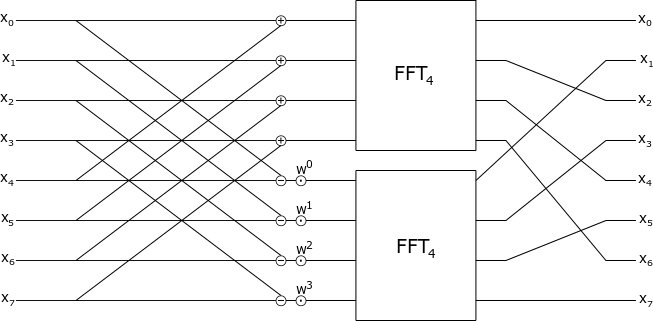
\includegraphics[width=0.8\textwidth]{Pictures/FFT.png}
\caption{Schmetterlingsdiagramm}
\label{fig:schmetterlingsdiagram}
\end{figure} 
Hier zu erkennen, dass am Ende die Elemente noch richtig sortiert werden müssen. 

\section{3D FFT}
Die 3 dimensionale FFT (3D FFT) wird in vielen verschiedenen Anwendungsbereichen benötigt.
In der Molekulardynamik zum Beispiel werden Simulationen von den physikalischen Bewegungen der Atome und Moleküle durchgeführt. Mit Hilfe des 3D FFT wird die Komplexität dieser Simulation verringert \cite[S.1]{shahe 14}.
\newline
Die 3D DFT ist definiert als \cite[S.4]{sig 07}:
\begin{equation}
F(k_x,k_y, k_z)= \sum_{j_x=0}^{N-1} \sum_{j_y=0}^{N-1} \sum_{j_x=0}^{N-1} 
f(j_x,j_y, j_z) e^{-2 \pi i \left( \frac{k_x j_x}{N_x} + \frac{k_y j_y}{N_y} + \frac{k_z j_z}{N_z} \right)}
\label{3dfft}
\end{equation}
Hierbei ist $f(x, y, z)$ ein 3 dimensionales Input-Array mit der Größe $N_x * N_y * N_z$ und $F(k_x,k_y, k_z)$ ein 3 dimensionales Output-Array.
Formel \ref{3dfft} kann in die folgende Form umgeschrieben werden:
\begin{equation}
F(k_x,k_y, k_z)= \sum_{j_x=0}^{N-1} \left( \sum_{j_y=0}^{N-1} \left( \sum_{j_x=0}^{N-1} 
f(j_x,j_y, j_z) e^{-2 \pi i \left( \frac{k_z j_z}{N_z} \right)} \right) e^{-2 \pi i \left( \frac{k_y j_y}{N_y} \right)} \right) e^{-2 \pi i \left( \frac{k_x j_x}{N_x} \right)}
\end{equation}
Dies zeigt das der drei dimensionale Fall als drei seperate ein dimesionale DFT berechent werden kann. Zuerst wird die DFT über die Z-Dimension berechnet. Dies führt zu folgenden Resultat:
\begin{equation}
F(j_x,j_y, k_z)=\sum_{j_x=0}^{N-1} 
f(j_x,j_y, j_z) e^{-2 \pi i \left( \frac{k_z j_z}{N_z} \right)}
\label{eq3dz}
\end{equation}
Die gleiche Methode wird auf die Y-Dimenstion angewendet:
\begin{equation}
F(j_x,k_y, k_z)=\sum_{j_x=0}^{N-1} 
f(j_x,j_y, j_z) e^{-2 \pi i \left( \frac{k_y j_y}{N_y} \right)}
\label{eq3dy}
\end{equation}
Zum Schluss wird noch die X-Dimension berechnet:
\begin{equation}
F(k_x,k_y, k_z)=\sum_{j_x=0}^{N-1} 
f(j_x,j_y, j_z) e^{-2 \pi i \left( \frac{k_x j_x}{N_x} \right)}
\label{eq3dx}
\end{equation}
Die Reihenfolge der Dimensionen ist nicht relevant für die 3D DFT \cite[S.3-4]{sig 07}.
Die einzelnen 1D DFT können nun mit dem 1D FFT berechnet werden.

\section{FFT-ECP Implementierung}
Das FFT-ECP Projekt soll eine nachhaltige 3D FFT Bibliothek für verteilte-heterogene parallele Systeme zur Verfügung stellen. Dies wird von dem Exascale Computing Project (ECP), welches vom US Department of Energy finanziert wird, entwickelt \cite[S. 1]{sha 19}. 
\newline
FFT-ECP basiert auf FFTMPI, eine CPU-FFT Bibliothek, die von dem Sandia National Laboratory entwickelt wurde. Diese Bibliothek kann 3D- oder 2D-FFTs parallel auf verteilten Prozessoren durchführen. Momentan werden GPUs nicht unterstützt. Ein wichtiges Feature von FFTMPI ist die Flexilibität des Input- und Output-Layers \cite[S.2]{sha 19}. 
\newline
Der Algorithmus für die 3D FFT schaut wie folgt aus:
\newline
Der 3D FFT Algorithmus basiert auf der sogenannten Pencil decomposition \cite[S.1-2]{aya 19}.
Die Input-Daten sind ein 3D Tensor mit folgende Dimensionen $N_{x} * N_{y} * N_{z}$ (siehe Abb. \ref{fig:pencildecomposition} a). Die Daten werden auf einem Gitter von $P$ Prozessen verteilt, $P=P_0 * P_1 * P_1$. Wie im vorherigen Kapitel beschrieben, kann die 3D FFT in drei seperate 1D FFT aufgeteilt werden. Dazu müssen die Daten in sogenannte Pencils umgeformt werden. 
\newline
Im ersten Schritt werden die Pencils entlang der X-Achse geformt (siehe Abb. \ref{fig:pencildecomposition} b). Die Pencils werden auf die $P$ Prozesse verteilt und mit 1D FFTs berechnet. Es müssen $N_y * N_{z}$ FFTs berechnet werden. Danach müssen die Daten wieder umgeformt werden. 
\newline
Im zweiten Schritt werden Pencils entlang der Y-Achse gebildet (siehe Abb. \ref{fig:pencildecomposition} c). Die Pencils werden wieder auf die $P$ Prozesse verteilt und es werden $N_x * N_z$ 1D FFTs berechnet. 
\newline
Im dritten Schritt werden die Daten in Pencils entlang der Z-Achse umgeformt, verteilt und $N_x * N_y$ 1D FFTs berechnet (siehe Abb. \ref{fig:pencildecomposition} d). Zum Schluss werden die Daten noch einmal umgeformt, um sie in die Originalform zu bringen. 
\newline
Der Algorithmus benötigt somit 4 Phasen zum Umformen der Daten und 3 Phasen zum Berechnen der 1D FFTs. Das Umformen der Daten basiert auf dem Message Passing Interface(MPI). Die 1D FFTs werden von externen Bibliotheken berechnet.

\begin{figure}
\centering
 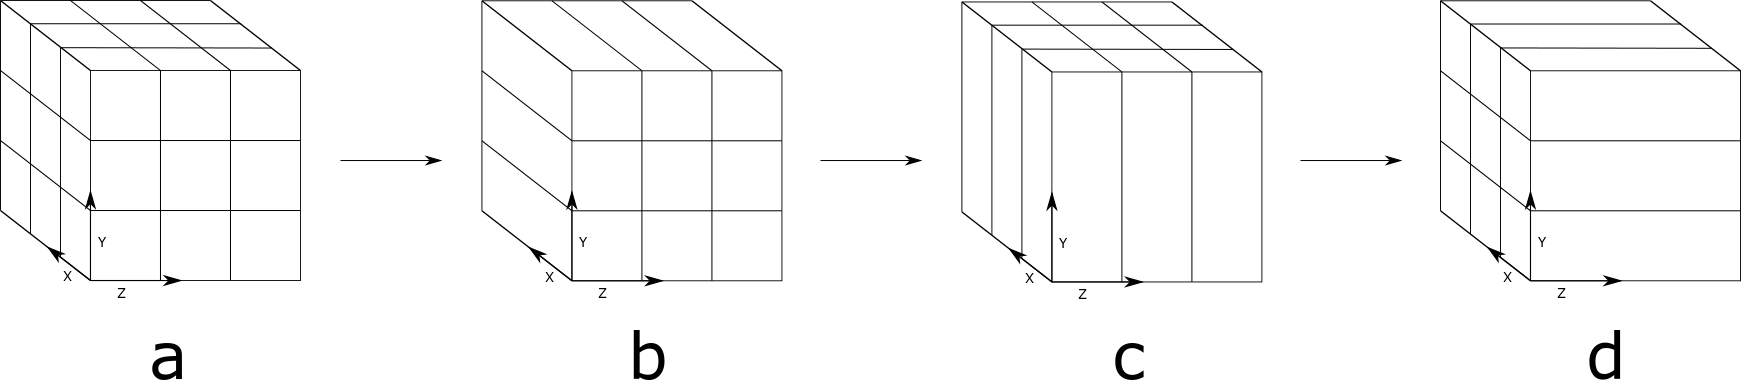
\includegraphics[width=0.8\textwidth]{Pictures/PencilsDecomposition.png}
\caption{Pencil Decomposition}
\label{fig:pencildecomposition}
\end{figure} 






\section{Kommunikationskostenoptimierung}
\hyphenation{High--Per-for-mance}
\hyphenation{Per-for-mance}
\hyphenation{Com-pu-ting}
\hyphenation{Be-rech-nungs-eng-pass}
Das Papier \cite{mainpaper} beschreibt in seinem dritten Kapitel Strategien zur Reduktion von Kommunikationskosten. Motiviert wird dies durch die Ergebnisse aus der Erfolgreichen GPU-Beschleunigung aus Kapitel 2.
Wie \cite[Abb. 3]{mainpaper} zeigt hat sich die Zeit, welche im FFT-Algorithmus f"ur Kommunikation zwischen den GPU's/CPU's aufgewendet wird, nur vernachl"assigbar ver"andert. Alle anderen Aktionen (Unpacking, Processing, Packing) haben sich erheblich durch Parallelisierung mit GPUs beschleunigt ($ \frac{0.74s}{0.017s} \approx 43.5$-fache Beschleunigung ).\\

Ein Berechnungsengpass durch Kommunikation von Applikationen in High-Performance-Computing(HPC)-Projekten, welche mehrere Prozessoren involvieren, scheint ein h"aufiges und bekanntes Problem zu sein.
%TODO quote references to similar bottlenecked projects
Dies kann dadurch begr"undet werden, dass Kommunikation "ublichweise genau dann unvermeidbar ist, wenn rein serielle Anteile in der Applikation/im Algorithmus present sind. Solche rein seriellen Anteile sind nicht parallelisierbar und ihre ergebnisse werden f"ur weitere Schritte ben"otigt, was Kommunikation in Multi-Prozessor-Systemen unvermeidbar macht.\\
%TODO cite sources
Um die Kommunikationskosten weiter zu optimieren steht eine Mischung aus folgenden Optionen zur Verf"ugung:
\begin{enumerate}
	\item Verwendung eines besseren Algorithmus hinsichtlich serieller Anteile und Kommunikation.
	\item Verbesserung der Kommunikationsstrategie unter Einbeziehung von Eigenschaften der Systemarchitektur.
\end{enumerate}

Die Schnelle Fouriertransformation (FFT) ist ein sehr spezifischer Algorithmus, was Verfolgungsm"oglichkeiten von Option 1 stark einschr"ankt. Dies mag der Grund daf"ur sein, weshalb sich \cite{mainpaper} auf Option 2 konzentriert.

\subsection{Relevante Technologien}
Das Papier benennt einige verwendete Technologien, gibt jedoch selbst dem Leser oft wenig Kontext zu diesen. Deshalb wird im Folgenden zu diesen Technologien der Kontext hergestellt.

\subsubsection{ NVIDIA GPUDirect }
	ist eine Technologie, die den direkten Zugriff von P"aripherie auf den Speicher von NVIDIA GPU's zul"asst. Dieser Vorgang wird als \textit{Remote Direct Memory Access} bezeichnet (RDMA).
		Dadurch wird der Umweg "uber traditionellen RAM vermieden. Beispiele für P"aripherien sind Netzwerkadapter, Speicher (wie Solid State Drives) und andere Graphikkarten. Es ist letztere Eigenschaft, welche im Kontext des Papiers vorrangig von Bedeutung ist (vgl. \cite{gpud}).

\subsubsection{ \textit{Message Passing Interface} (MPI) }
MPI ist ein Standard, der eine Schnittstelle für Nachrichten zwischen Prozessen spezifiziert. Portabilität und Einfachheit werden als prim"are Ziele angegeben (vgl. \cite[Kap. 1.1]{mpi}). Es gibt mehrere Implementierungen dieses Standards, zum Beispiel die Open-Source-Variante OpenMPI (\cite{openmpi}).

In verteilten Systemen wird MPI als Abstraktion für die Kommunikation zwischen parallelen Prozessoren/Prozessen verwendet.

\subsubsection{ CUDA }
Die \textit{\textbf{C}ompute \textbf{U}nified \textbf{D}evice \textbf{A}rchitecture}, entwickelt von NVIDIA ist eine Plattform und Programmiermodell f"ur parallele Computation auf NVIDIA GPUs. 

\subsubsection{ CUDA-aware MPI }
Ist eine Kombination aus CUDA und MPI. Da CUDA mit dem MPI Standard kompatibel ist, sind MPI-Implementierungen möglich, welche bessere Umsetzungen von MPI-Software auf NVIDIA GPUs erm"oglichen.

\subsection{Weitere Spezielle Terminologie}
\subsubsection{Sockel \textit{(eng. socket)}}
Ein Sockel fasst im Kontext von \cite{mainpaper} mehrere Prozessoren zusammen. Diese Zusammenfassung bringt, verursacht durch die Systemarchitektur, spezielle Eigenschaften bei Relationen der Prozessoren untereinander (hier: verfügbare Kommunikationstechnologie).\\
Folgende Terminologie wird dabei verwendet:
\begin{defi}[\textit{same-socket-communication}]
Ein Kommunikationsvorgang, welcher zwischen zwei Prozessoren unter dem selben Sockel erfolgt.
\end{defi}
\begin{defi}[\textit{cross-socket-communication}]
Ein Kommunikationsvorgang, welcher zwischen zwei Prozessoren erfolgt, welche sich nicht gemeinsam auf einem Sockel befinden.
\end{defi}

\subsubsection{Kommunikationsrichtung}
\begin{defi}[Unidirektionale Kommunikation (\textit{ eng. unidirectional communication })]
In einem abgeschlossenen Kommunikationsvorgang zwischen $p1$ und $p2$ werden Daten ausschlie"sslich von $p1$ nach $p2$ kommuniziert.
\end{defi}
\begin{defi}[Bidirektionale Kommunikation (\textit{ eng. bidirectional communication })]
In einem abgeschlossenen Kommunikationsvorgang zwischen $p1$ und $p2$ können Daten sowohl von $p1$ nach $p2$, als auch von $p2$ nach $p1$ ausgetauscht werden.
\end{defi}


\subsection{Systemarchitektur}
\cite[Abb. 1]{mainpaper} zeigt die generelle Systemarchitektur des Summit Supercomputers in Oak Ridge National Laboratory(ORNL), zu dem sich die vorgestellten Überlegungen im Papier zu relativieren scheinen. Die Grafik zeigt Knoten, welche "uber verschiedene Arten von Networking/Bussen verbunden sind. Diese verschiedenen Networking-Technologien gehen mit verschiedenen Übertragungseigenschaften (vorrangig Bandbreite einher). Ebenfalls zu erkennen is das Konzept eines Sockels (\textit{eng. socket}), welcher mehrere Prozessoren zusammenfasst. 

Innerhalb eines Sockels sind alle Prozessoren (7TF GPU's) Peer-to-Peer "uber die NVLINK Technologie verbunden (50GB/s Bandbreite). Same-Socket kommunikation k"onnte netzwerktopologisch also Gesamtinformation mit einer Bandbreite von $50Gb/s * \frac{p^2}{2}$ austauschen (Mit $p$ als die Anzahl der beteiligten Prozessoren auf dem Sockel).
%TODO check if with NVLINK 50Gb is the speed set for bidirectional communication
Zwischen den Sockeln exisitiert ein X-Bus (64GB/s).
Theoretisch k"onnen also maximal $\frac{64GB/s}{50GB/s} = 1.28$ Prozessoren cross-socket kommunizerien. Unter der Annahme, dass jeder Prozess im Schnitt mit jedem anderen Prozess gleich viel kommuniziert  entstehen demnach Kommunikationsengp"asse zuerst bei der cross-socket Kommunikation.\\
Bestimmte Kommunikationsstrategien verhalten sich also besser auf bestimmten Zielarchitekturen als andere.
\cite{mainpaper} versucht deshalb durch Benchmarking zu optimieren. 

\subsection{Benchmarking}


\section{Zusammenfassung}
Die schnelle Fouriertransformation verringert die Laufzeit der diskreten Fouriertransformation von $\mathcal O(n^2)$ auf $\mathcal O(n \log n)$. Da 3D-FFTs mit Hilfe von 1D-FFTs berechnet werden, wird die Laufzeit der  3D-Fouriertransformation ebenfalls verringert. 
\newline
Durch die Verwendung von GPUs anstatt CPUs und massiver Parallelität ist eine bis zu 40-fache Beschleunigung der 3D-FFTs möglich. Durch diese Beschleunigung der Berechnung wird Kommunikation im Multi-Prozessorsystem jedoch zum Berechnungsengpass. Dieser Engpass kann durch eine geeignete Wahl der Kommunikationsstrategie und vorteilhafte Änderung des verwendeten Algorithmus für bessere Kommunikationseigenschaften mitigiert werden.



\newpage

\begin{thebibliography}{12}
%\bibitem[HaKT1 98]{HaKT1 98} \footnote{In die 
%Bibliographie sollte s"amtliche benutzte Literatur 
%rein, auch nicht beim eigenen Vortrag angegebene, aber benutzte Papiere 
%und B\"ucher. Gleichzeitig sollte aber alles in der Literaturliste angegebene
%mindestens einmal im Artikel zitiert werden, sonst nicht auflisten.}
        %Michael Harkavy, J. D. Tygar, Hiroaki Kikuchi: {\sl Multi-round 
        %Anonymous Auction Protocols}; 1st IEEE Workshop on Dependable and 
        %Real-Time E-Commerce Systems, 1998.

%Here go sources, which both grr and tse might need
% for example

%the subject paper
\bibitem[ShaH19]{mainpaper}
		Shajek H., Tomov S., Ayala A., Haidar A., Dongarra J: {\sl GPUDirect MPI Communications and Optimizations to Accelerate FFTs on Exascale Systems}
		EuroMPI ’19 Posters, September 11-13, 2019, Zurich, Switzerland

\bibitem[GrrDef\_79]{grr}
        Graf Default: {\sl How to Cite something}; 
        Communications of the ACM 22/11 (1979), S. 612-613.

\bibitem[NV\_GPUD]{gpud}
		NVIDIA: {\sl GPUDirect};
		\url{https://developer.nvidia.com/gpudirect}; Zuletzt aufgerufen: 2019-11-24


\bibitem[MPI12]{mpi}
		Message Passing Interface Forum: {\sl MPI: A Message-Passing Interface Standard Version 3.0}; 2012-09-21
		University of Tennessee, Knoxville, Tennessee

\bibitem[OpenMPI]{openmpi}
		OpenMPI: {\sl OpenMPI}
		\url{https://www.open-mpi.org} ; Zuletzt aufgerufen: 2019-11-24

\bibitem[MPImanpage]{MPImanpage}
		Open MPI: {\sl MPI\_Alltoall(3) man page (version 1.8.8)};
		The Open MPI Project; 2019-05-20
		\url {https://www.open-mpi.org/doc/v1.8/}; Zuletzt aufgerufen: 2019-12-16

\bibitem[NV\_CUDA]{cuda}
		CUDA-Zone: {\sl CUDA}
		\url{https://developer.nvidia.com/cuda-zone}; Zuletzt aufgerufen: 2019-11-24

\bibitem[NV\_CUDAMPI]{cudampi}
		Kraus, Jiri: {\sl An Introduction to CUDA-Aware MPI};
		NVIDIA Developer Blog; 2013-05-13;	
		\url{https://devblogs.nvidia.com/introduction-cuda-aware-mpi/}; Zuletzt aufgerufen: 2019-11-24

\bibitem[NV\_Summit]{summit}
		Foertter, Fernanda; {\sl Summit GPU Supercomputer Enables Smarter Science}; NVIDIA Developer Blog; 2018-06-08
		\url{https://devblogs.nvidia.com/summit-gpu-supercomputer-enables-smarter-science/}; Zuletzt aufgerufen: 2019-12-21

\bibitem[OLCF\_Summit]{osummit}
		Oak Ridge National Laboratory:{\sl SUMMIT, Oak Ridge National Laboratory's 200 petaflop supercomputer}
		\url{https://www.olcf.ornl.gov/olcf-resources/compute-systems/summit/}; Zuletzt aufgerufen: 2020-01-06

\bibitem[NVLINK]{nvlink}
	NVLink NVIDIA;
	\url{https://en.wikichip.org/wiki/nvidia/nvlink}; Zuletzt aufgerufen: 2020-01-12

\bibitem[FatTree]{fattree}
		Solnushkin, Konstantin: {\sl Fat-Tree Design}
		\url{https://clusterdesign.org/fat-trees/}; Zuletzt aufgerufen: 2020-01-06

%[HeJoBu 84]
\bibitem[2] {hejobu 84} M. Heideman, D. Johnson and C. Burrus: {\sl Gauss and the history of the fast fourier transform}; IEEE ASSP Magazine, vol. 1, no. 4, October 1984.
%[KreNor 11]
\bibitem[3] {krenor 11} E. Kreyszig, H. Kreyszig, und E. Norminton: {\sl Advanced Engineering Mathematics}; Wiley, 10 Edition, 2011.
%[Scho 05]
\bibitem[4] {scho 05} Arthur L. Schoenstadt: {\sl An Introduction to Fourier Analysis Fourier Series, Partial Differential Equations
and Fourier Transforms
}; Department of Applied Mathematics Naval Postgraduate School, 2005.
%[Ser 17]
\bibitem[5] {ser 17} Valery Serov: {\sl Fourier Series, Fourier Transform and Their Applications to Mathematical Physics}; Springer Verlag, 2017.
%[Sig 07]
\bibitem[6] {sig 07} U. Sigrist: {\sl “Optimizing parallel 3D fast Fourier transformations for a
cluster of IBM POWER5 SMP nodes}; Ph.D. Dissertation, The University of Edinburgh, Aug 2007.
%[SHaHe 14]
\bibitem[7] {shahe 14}J. Sheng, B. Humphries, H. Zhang and M. C. Herbordt: {\sl Design of 3D FFTs with FPGA Clusters}; IEEE High Performance Extreme Computing Conference (HPEC), 2014.
%[Aya 19]
\bibitem[8] {aya 19} Ayala A., S. Tomov, X. Luo, H. Shaiek, A. Haidar, G. Bosilca, and J. Dongarra: {\sl Impacts of Multi-GPU MPI Collective Communications on Large FFT Computation}; Workshop on Exascale MPI (ExaMPI) at SC19, 2019.
%[And 12]
\bibitem[9] {and 12}André Neubauer: {\sl DFT – Diskrete Fourier-Transformation Elementare Einführung}; Springer Vieweg, 2012

\end{thebibliography}
\end{document}





